
% titlepage-demo.tex
\documentclass{beamer}
\usetheme{Boadilla}
\usepackage{multirow}
\usepackage[absolute,overlay]{textpos} 
\newenvironment{reference}[2]{% 
  \begin{textblock*}{\textwidth}(#1,#2) 
      \footnotesize\it\bgroup\color{red!50!black}}{\egroup\end{textblock*}} 

\begin{document}

%\begin{frame}[t]{Video-based Approach}
%Bag-of-visual-words model: Video level features are aggregated over the entire videos

%\begin{center}
%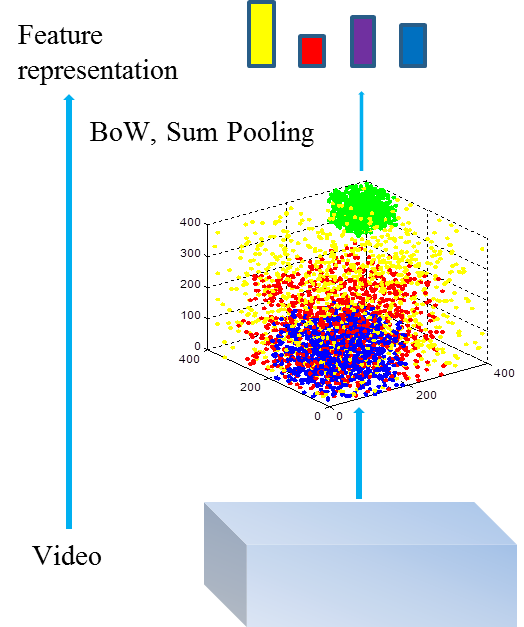
\includegraphics[width=5cm,height=4.5cm]{images/video_based_summax.png}
%\end{center}

%\begin{itemize}
%\item The proposed segment-based approach: increasing the number of segment representation is not scalable. 
%\item \textbf{Specific problem:} How to generate one representation per each video from its segment-level representations?
%\end{itemize}

%\end{frame}

\begin{frame}[t]{How to Detect Event in Video?}
	\begin{itemize}
		\item State-of-the-art systems [Jiang - TRECVID2010], [Natarajan - TRECVID2011] (\textbf{best systems} in TRECVID MED 2010 and 2011)
	\end{itemize}
	
	\begin{center}
		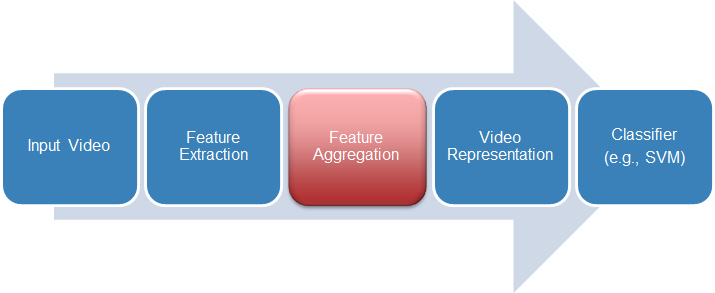
\includegraphics[width=10cm,height=4cm]{images/part3/standardapproach.png}
	\end{center}
	
		\textbf{Problem}: Neutralize the contribution of each part of the whole video. 
		\begin{itemize}
			\item In fact, the clues to determine an event often appear in a small segment.
		\end{itemize}
		
\end{frame}

\begin{frame}[t]{How to Aggregate Feature?}
	\begin{itemize}
		\item \textbf{Sum pooling} strategy [Jiang TRECVID2010], [Natarajan TRECVID2011] (\textbf{best systems} in TRECVID MED 2010 and 2011).
		\begin{itemize}
\item dominant by frequently-occurring descriptors
\item rarely occurring descriptors have less influential
		\end{itemize}	
		
		\item \textbf{Max pooling} strategy [Wang ACCV2012] (often used with sparse coding for image classification [Yang CVPR2009])
				\begin{itemize}
					\item only select the most discriminative information
					\item likely to lost other crucial information
				\end{itemize}	
		\item \textbf{Dynamic pooling} [Li ICCV2013]: dynamically
		determine the pooling operator most suited for each
		sequence using Latent SVM. \\
		$\rightarrow$ very time-consuming!
			
	\end{itemize}
	Problem: How to combine \textbf{Sum pooling} and \textbf{Max pooling} in a efficient way?


\end{frame}

\begin{frame}{Sum-max Video Pooling} 
	\begin{itemize}
\item \textbf{Sum pooling} at lower layer to accumulate sufficient features.
\item \textbf{Max pooling} to retrieve the most relevant features at the high layer.
$\rightarrow$ can discard irrelevant features in the final video representation.
%\bigskip
	\end{itemize}

\begin{columns}
  \begin{column}{0.3\textwidth}
    \centerline{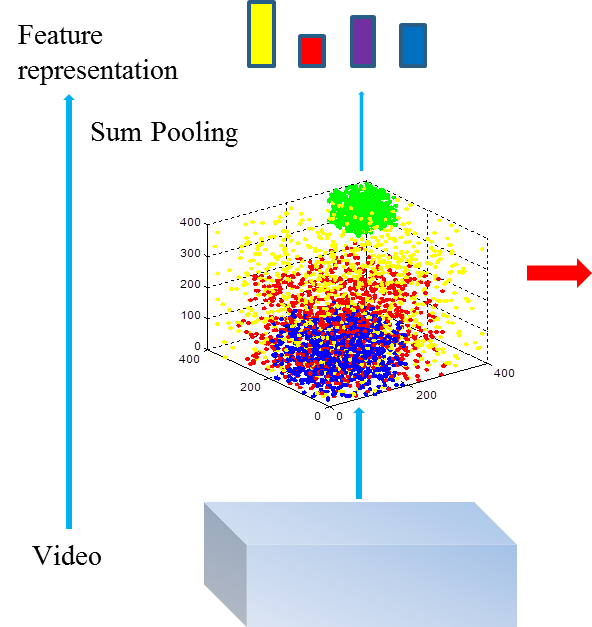
\includegraphics[width=1\textwidth]{images/video_based_summax2.png}}
    (a) The video-based approach
  \end{column}

  \begin{column}{0.7\textwidth}
    \centerline{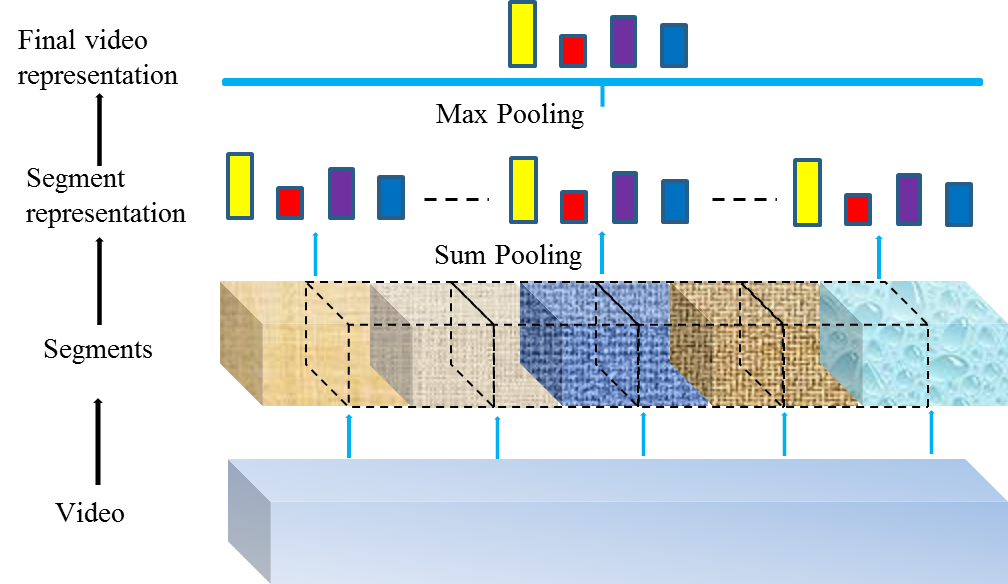
\includegraphics[width=1\textwidth]{images/segment_based_summax.png}}
    (b) \textbf{Our proposed Sum-max Video Pooling}
  \end{column}
\end{columns}
\bigskip
 
  
\end{frame}

\begin{frame}[t]{Sum-max Video Pooling}

\begin{itemize}
	\item Notation:
\begin{itemize}
\item N local descriptors $x_{n} \in R^{D}$, n = 1,...,N and D is the feature dimension
\item K visual words $m_{k} \in R^{D}$, where k = 1,...,K 
\item $M = \{m_{k}\}$ is the set of visual words
\item Coding step: $\phi_{n} = [\Phi_{1n},...,\Phi_{Kn}]$
\item \textit{S} is number of segments
\item $N_{s}$ is the number of local descriptors in segment \textit{s} 
\end{itemize}
\item The sum-max and max-sum video pooling at each visual word can be defined as follows:
\begin{equation}\psi_{k_{\textbf{sum-max}}} = Max_{s \in S}(\sum_{n \in N_{s}}\Phi_{kn})\end{equation}

\begin{equation}\psi_{k_{\textbf{max-sum}}} = \sum_{s \in S}(Max_{n \in N_{s}}\Phi_{kn})\end{equation}
\end{itemize}

\end{frame}

\begin{frame}[t]{Complexity}
	
	\begin{itemize}
		\item Same complexity with the \textbf{sum video pooling}:
		\begin{equation}\psi_{k_{\textbf{sum-max}}} = Max_{s \in S}(\sum_{n \in N_{s}}\Phi_{kn})\end{equation}
		
		\begin{equation}\psi_{k_{\textbf{sum}}} = \sum_{s \in S}(\sum_{n \in N_{s}}\Phi_{kn})\end{equation}
		\item Very efficient
	 	\begin{itemize}
	 		\item Extracting features only once!
	 		\item Aggregating features at different segment lengths efficiently.
		\end{itemize}
	\end{itemize}
		\begin{center}
			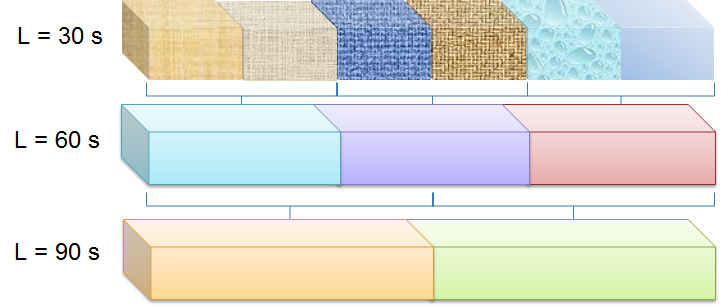
\includegraphics[width=8cm,height=3cm]{images/part3/efficient.png}
			\\	\scriptsize{Features from higher layers can be obtained from lower layers efficiently!}
		\end{center}
\end{frame}

\begin{frame}{Experimental Setup} 	
	\begin{itemize}
		\item Dataset
		
		\begin{table}[h]
			\tiny
			\begin{tabular}{@{}|l|c|c|c|c|c|@{}}
				\toprule
				\multicolumn{1}{|c|}{Dataset} & No. Event & No. Train Videos & No. Test Videos & Total Videos & Total Hours \\ \midrule
				MED2010 & 3 & 1,744 & 1,724 & 3,468 & 110 hours \\ \midrule
				MED2011 & 10 & 1,331 & 31,822 & 33,153 & 1,100 hours \\ \midrule
				\light{MED2012} & \light{25} & \light{3,878} & \light{1,938} & \light{5,816} & \light{250 hours} \\ \bottomrule
			\end{tabular}
		\end{table}
		
		\item Feature: 
			\begin{itemize}
				\item MED10: Dense Trajectories, MBH descriptor [Wang-CVPR2011] 	
				\item MED11: Improved Dense Trajectories, MBH descriptor [Wang-ICCV2013] 	
			\end{itemize}
		\item Feature encoding: Bag-of-words model, 4000 codewords.
		\item Learning: ${\chi}^{2}$ SVM.
	\end{itemize}
	
\end{frame}	

\begin{frame}[t]{Experimental Results: On MED 2010}
\begin{table}
\renewcommand{\arraystretch}{1}
\caption{Performance comparison of different video pooling strategies on the MED 2010 dataset.}
\label{t_med10}
\centering
\begin{tabular}{|c|c|c|c|c|}
\toprule
Event/MAP & \begin{tabular}[x]{@{}c@{}}Max pooling\\(Video-based) \end{tabular} & \begin{tabular}[x]{@{}c@{}}Sum pooling\\(Video-based) \end{tabular} & \begin{tabular}[x]{@{}c@{}}Max-sum\\pooling\\(at 60 s)\end{tabular} & \begin{tabular}[x]{@{}c@{}}Sum-max\\pooling\\(at 60 s)\end{tabular} \\
%\bfseries \begin{tabular}[c]{@{}c@{}} CU\\(SIFT)\end{tabular}&
%\bfseries \begin{tabular}[c]{@{}c@{}}CU (STIP,\\SIFT,\\MFCC)\end{tabular}\\
\midrule
E001&0.4365&0.4468&0.4646&\textbf{0.5072}
\\
\midrule
E002&0.6434&\textbf{0.7988}&0.7103&0.7900
\\
\midrule
E003&\textbf{0.3144}&0.3053&0.2806&0.3100
\\
\midrule
All&0.4648&0.5170&0.4852&\textbf{0.5357}
%&0.512&0.633
\\
\bottomrule
\end{tabular}
\end{table}


\begin{itemize}
\item Pooling over segments is more effective.
\item \textbf{Sum-max video pooling outperforms the traditional video-based sum pooling.}
\end{itemize}
\end{frame}

\begin{frame}[t]{Experimental Results: On MED 2011}
\begin{center}
	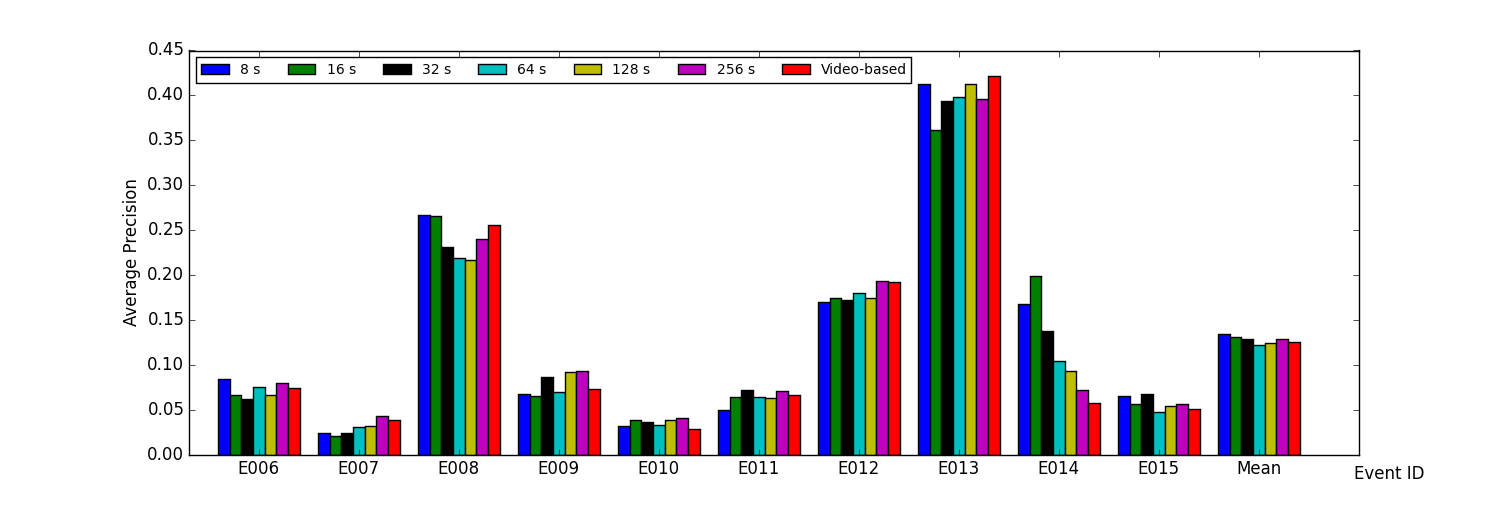
\includegraphics[width=12cm,height=3.5cm]{images/part3/med11_summax_kernel2.png}
	\\	\scriptsize{Results of Sum-max video pooling on the MED 2011 dataset.}

\begin{table}[h]
	\tiny
	\begin{tabular}{@{}|c|c|c|c|c|c|c|c|@{}}
		\toprule
		Method/mAP                                                                   & 8 s       & 16 s      & 32 s   & 64 s   & 128 s  & 256 s  & video-based \\ \midrule
		Sum-Max                                                                      & \textbf{0.1339}    & 0.1311   & 0.1282 & 0.1220 & 0.1242 & 0.1283 & 0.1257      \\ \midrule
		Segment-based                                                                & \multicolumn{2}{c|}{} & 0.1510 & 0.1503 & \textbf{0.1518} & 0.1365 & 0.1257      \\ \bottomrule
%		\begin{tabular}[c]{@{}c@{}}Dynamic Pooling \\ {[}Li-ICCV2013{]}\end{tabular} & \multicolumn{6}{c|}{}                                     & 0.1227      \\ \bottomrule
	\end{tabular}
\end{table}
	
\end{center}
\begin{itemize}
	\item The best performance is at 8 s (\textbf{6}\% improvement!)
	\item Sum-max video pooling performs significantly worse than the segment-based approach!
	\item However, sum-max video pooling is very \textbf{efficient}!
\end{itemize}

\end{frame}

\begin{frame}[t]{Conclusions}
	
	\begin{enumerate}
		\item \light{Segment-based Representation (SB)}
		\item \textbf{Sum-Max Video Aggregation (SM)}
		\begin{itemize}
			\item An efficient method to aggregate\\
			local features into video feature \\
			representation.
		\end{itemize}
		\item \light{Event-driven Multiple Instance \\
			Learning (EDMIL)}
	\end{enumerate}
	
	
	\begin{tikzpicture}[remember picture,overlay]  
	\node [xshift=-3cm,yshift=-4.5cm] at (current page.north east)
	{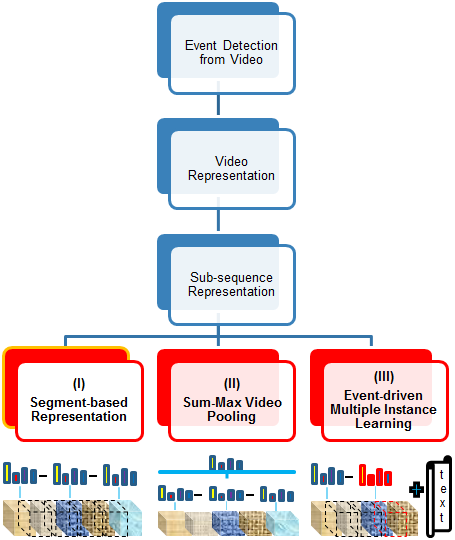
\includegraphics[width=5cm,height=7.5cm]{images/part1/contribution2.png}};
	\end{tikzpicture}
	
\end{frame}



\end{document}